\section{The PRNG}
The PRNG utilises SHA-256 as hash function.
The entropy pool is 64 bytes (512 bits) large, which is the block size of SHA-256.
We specify to algorithms which implement the functionality of the PRNG, one to add entropy to the entropy pool and one to get a block (32 bytes) of random data.
\begin{algorithm}
\caption{Add some data to the entropy pool}
\label{algAddEntropy}
\begin{algorithmic}
\REQUIRE $pool = pool_0 \parallel pool_1$ where $pool_0$ and $pool_1$ are both 32 bytes large
\REQUIRE $data$ of arbitrary length
\REQUIRE $offset$ which may be 0 or 1
\STATE $temp \leftarrow H(pool \parallel data)$
\STATE $pool_{offset} \leftarrow pool_{offset} \oplus temp$
\STATE $offset \leftarrow offset \oplus 1$
\end{algorithmic}
\end{algorithm}

\begin{algorithm}
\caption{Get a block of random from the entropy pool}
\label{algGetRandom}
\begin{algorithmic}
\REQUIRE $pool = pool_0 \parallel pool_1$ where $pool_0$ and $pool_1$ are both 32 bytes large
\REQUIRE $offset$ which may be 0 or 1
\STATE $temp \leftarrow H(pool)$
\STATE $pool_{offset} \leftarrow pool_{offset} \oplus temp$
\STATE $offset \leftarrow offset \oplus 1$
\STATE $temp[temp[0] \wedge 31] \leftarrow temp[temp[0] \wedge 31] + 1$
\STATE $OUTPUT \leftarrow H(temp)$
\end{algorithmic}
\end{algorithm}

\begin{figure}
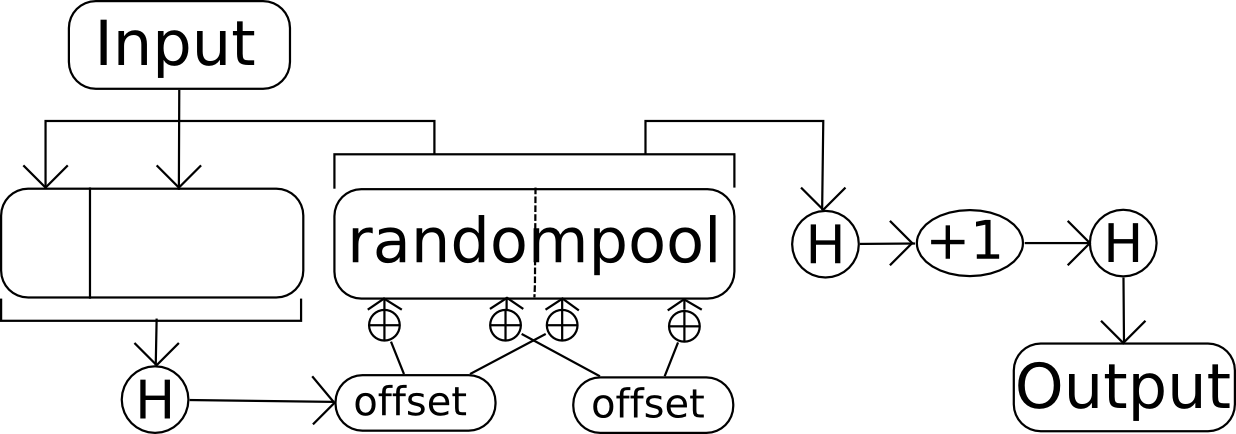
\includegraphics[scale=0.3]{PRNG} 
\caption{schematic of the PRNG}
\end{figure}